\documentclass[capstone_report.tex]{subfiles}
\begin{document}
\chapter*{Abstract}                                
The recent increase in the availability of small, battery powered, unmanned aircraft has created the opportunity for increased deployment in the emergency services industry. The Melbourne Metro Fire Brigade currently has a unmanned aerial vehicle (UAV) team which consists of a fleet of aircraft and pilots. To date, the role of this team has been limited to scenarios where the UAVs can be deployed outdoors, or after the fact as in forensic investigations.\\

Deployment of UAVs indoors is challenging for pilots due to a lack of line-of-sight to the UAV, and the very low margin of error given the prevalence of obstacles. At the same time, indoors presents one of the most hazardous situations for emergency personnel. It is therefore highly desirable to develop an automated UAV which can reduce the incidence of personnel being exposed to hazardous conditions without requiring precision piloting.\\

Our project aimed to design and build a prototype UAV which can enter an indoor environment, navigate autonomously, and generate a map of the area and live video feed. We show the design of an Unmanned Recon and Safety Aircraft (U.R.S.A.) which can navigate in a number of basic indoor environments without human interaction. The final product delivered consists of a UAV which can navigate and map in a real world indoor space. The primary mechanism of navigation is 2D laser scan data. Range measurements are taken in a \SI{240}{\degree} arc, and these are converted to a joint estimate of URSA's position and surrounding obstacles. A sampling approach is then used for pathfinding. Figure \ref{fig:sim} shows URSA in simulation, and Figure \ref{fig:real} shows the real-world prototype.\\ 

Results are presented in terms of both qualitative assessment of navigation performance in different environments, as well as a quantitative comparison of floor map measurements against ground truth data. In both metrics, URSA performs well. Areas for future investigation include controller refinement to allow faster execution of flight paths, and extension to 3D environment mapping.


    \begin{figure}  [H]
	\centering
        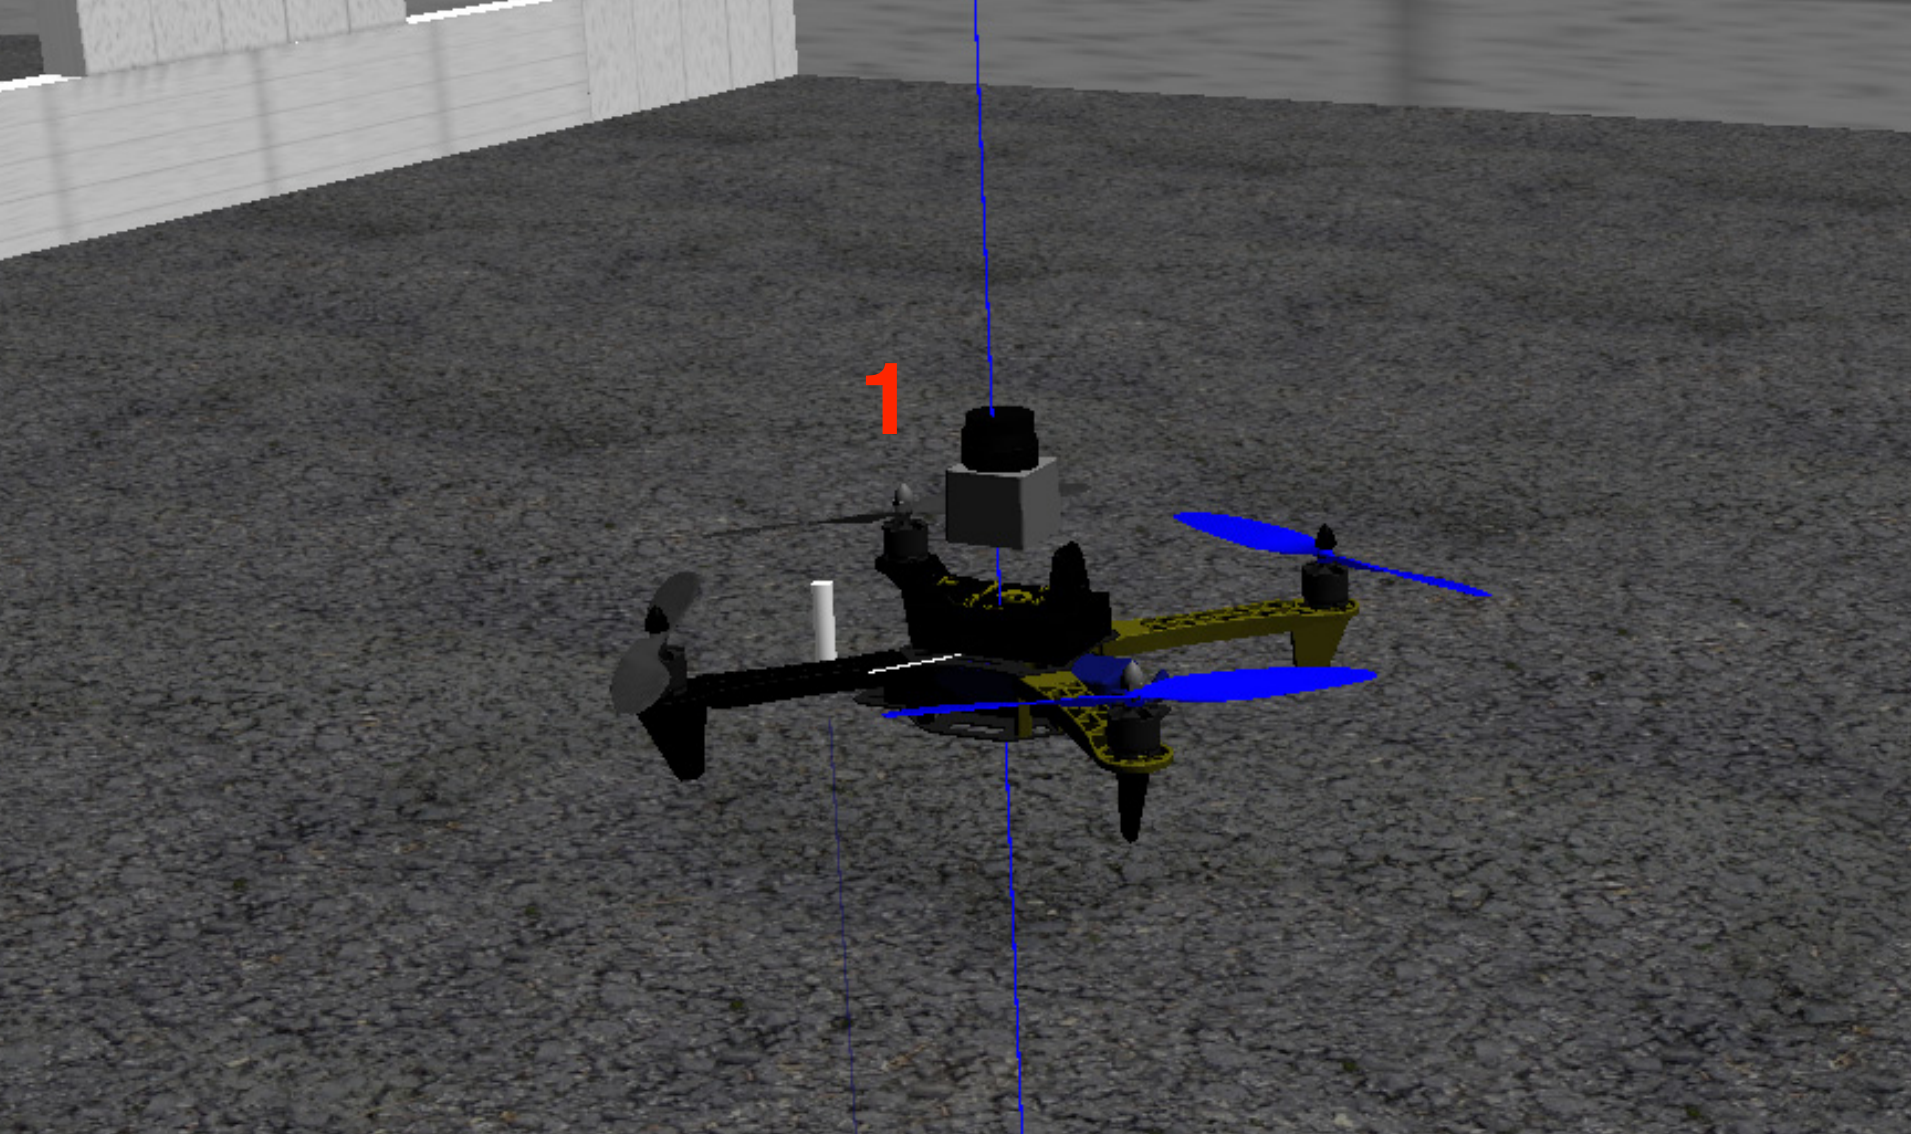
\includegraphics[width=0.6\linewidth]{imgs/simulation_labelled.png}
        \captionof{figure}{URSA in simulation. (1) LiDAR sensor}
        \label{fig:sim}
    \end{figure}


    \begin{figure}  [H]
	\centering
        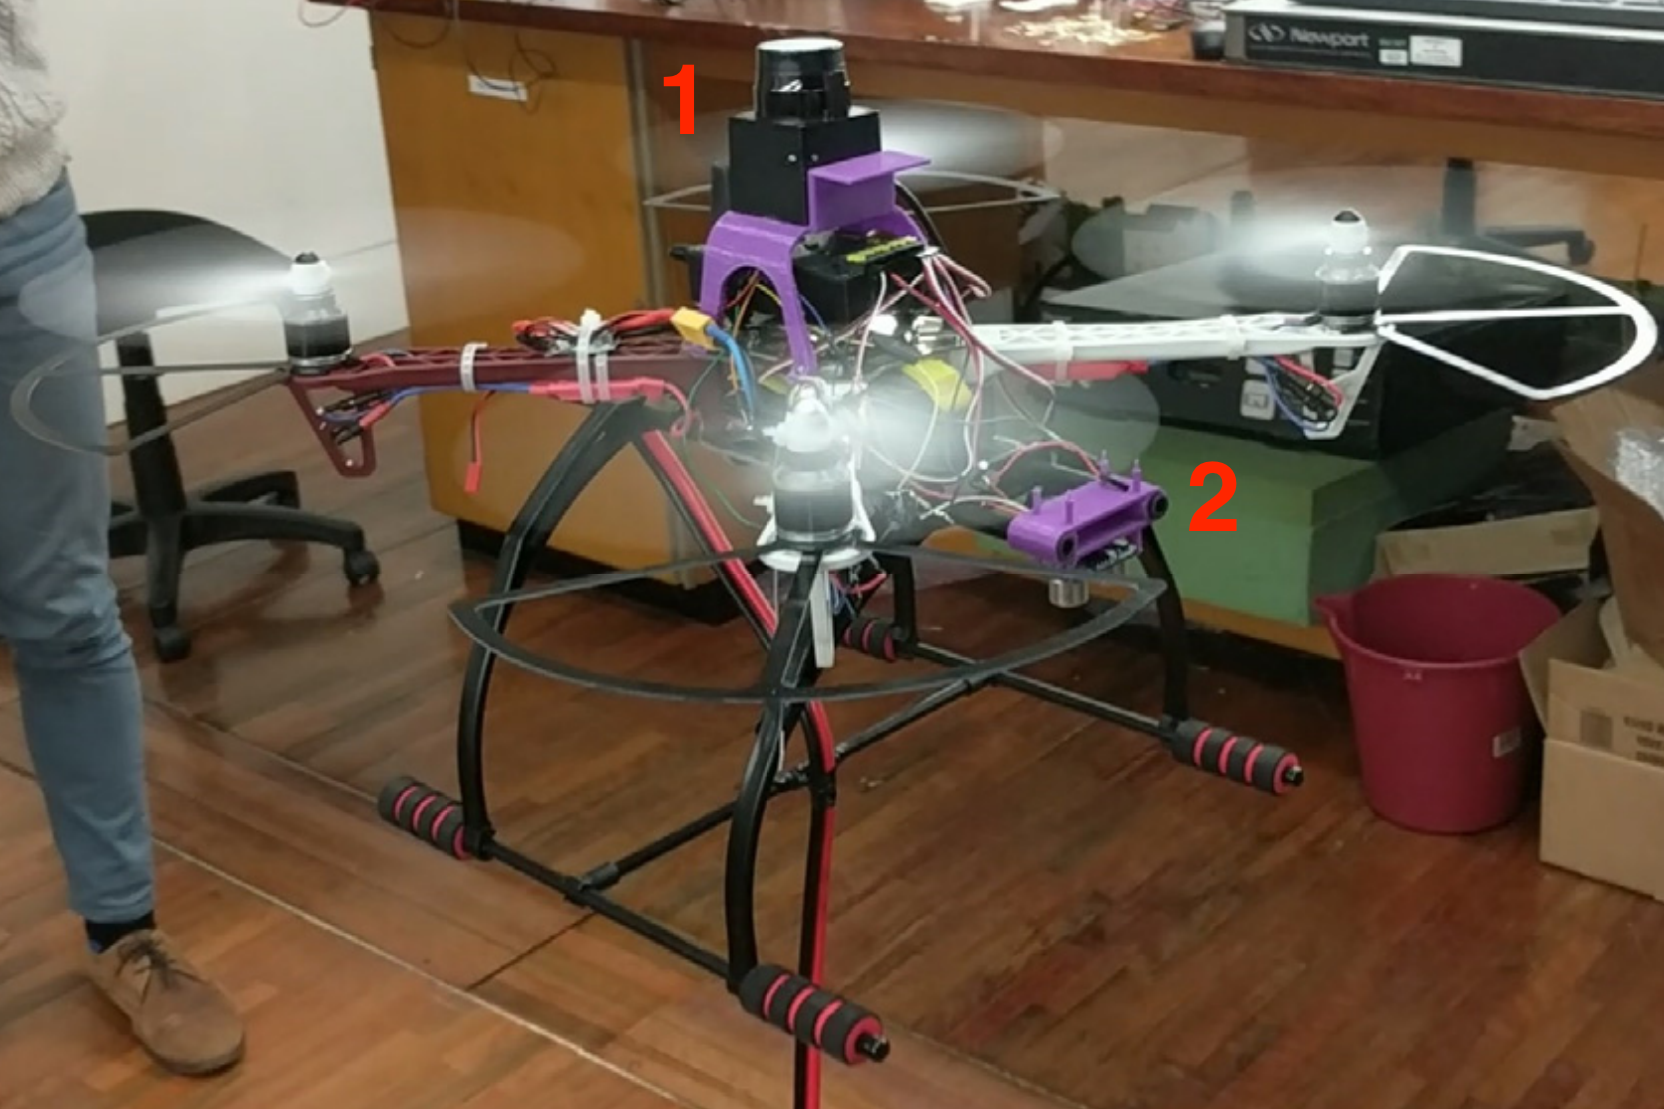
\includegraphics[width=0.6\linewidth]{imgs/real_labelled.png}
        \captionof{figure}{URSA real world prototype assembled from components. (1) LiDar sensor mounted on bracket designed by URSA (2) Ultrasonic sensor interfaced with signal conditioning PCB and bracket designed by URSA}
        \label{fig:real}
    \end{figure}

\end{document}